%%
%% Author: leigh-anne_mathieson
%% 2019-03-26
%%

% Preamble
\documentclass[11pt]{article}

% Packages
\usepackage{graphicx}
\usepackage{subcaption}
\usepackage{hyperref}
\usepackage{algorithm2e}
\graphicspath{ {./images/} }
% Document
\begin{document}

\section{Week 2 - Gradient Descent}
%    \subsection{Gradient Descent}

    We want to find $\theta_0$, $\theta_1$ that will minimise our cost function \[J(\theta_0, \theta_1) = \frac{1}{2m} \sum^m_{i=1}(h_\theta(x^{(i)}) - y^{(i)})^2\]

    We will use gradient descent to do that. Here is the idea: Imagine that you are in a hilly landscape blindfolded, and you want to get to the lowest elevation around. What would you do? You'd probably tap around your immediate area, and then move to the lowest elevation that you found. Then you'd repeat until you tapped around your immediate area and found that the ground around you to all be higher or on the same level. That is what gradient descent does.

    Our plan:
    \begin{itemize}
        \item Pick some $\theta_0, \theta_1$ (Perhaps $\theta_0=1, \theta_1=1$, but it doesn't really matter).
        \item Keep changing  $\theta_0, \theta_1$ to reduce $J(\theta_0, \theta_1)$, until we have found a minimum
    \end{itemize}

    More formally:
    
\begin{algorithm}
    \SetAlgoLined
    \KwData{ A set of points to which we are fitting a line $(x^{(1)}, y^{(1)}), (x^{(2)}, y^{(2)}), ... , (x^{(m)}, y^{(m)})$ }
    \KwResult{$\theta_0$, $\theta_1$, parameters for the line that fits the input data }
     set some initial values for $\theta_0, \theta_1$ \\
    
    \While{we have not reached convergence}{
    	\[\theta_0 := \theta_0 - \alpha \frac{\delta}{\delta \theta_0} J(\theta_0, \theta_1)\]

    	\[\theta_1 := \theta_1 - \alpha \frac{\delta}{\delta \theta_1} J(\theta_0, \theta_1)\]

	}

    \Return $\theta_0, \theta_1$

    \caption{algorithm for \textbf{gradient descent}}
\end{algorithm} 


    We will update  $\theta_0$, $\theta_1$ simultaneously.

    $\alpha$ is the learning rate, and it represents the size of the step you take in each iteration. More on that later.  $\frac{\delta}{\delta \theta_0} J(\theta_0, \theta_1) $ and $\frac{\delta}{\delta \theta_1} J(\theta_0, \theta_1) $ are partial derivatives for the cost function, and they represent the direction we need to go if we want $J(\theta_0, \theta_1)$ to decrease in the next iteration. Here is the algorithm with the partial derivatives for our cost function subbed in:
    
    
    \begin{algorithm}
    \SetAlgoLined
    \KwData{ A set of points to which we are fitting a line $(x^{(1)}, y^{(1)}), (x^{(2)}, y^{(2)}), ... , (x^{(m)}, y^{(m)})$ }
    \KwResult{$\theta_0$, $\theta_1$, parameters for the line that fits the input data }
     set some initial values for $\theta_0, \theta_1$ \\
    
    \While{we have not reached convergence}{
    	\[\theta_0 := \theta_0 - \alpha \frac{1}{m} \sum^m_{i=1} (h_\theta(x^{(i)}) - y^{(i)} )\]

   	 \[\theta_1 := \theta_1 - \alpha \frac{1}{m} \sum^m_{i=1} (h_\theta(x^{(i)}) - y^{(i)}) \times x^{(i)}\]
	}

    \Return $\theta_0, \theta_1$

    \caption{algorithm for \textbf{gradient descent}}
\end{algorithm} 
    
    \subsection{Gradient Descent - how do we detect convergence?}

    The number of iterations we need will vary, but note that:
    \begin{itemize}
        \item For sufficiently small $\alpha$, $J(\theta)$ should decrease on every iteration
        \item But if $\alpha$ is too small, gradient descent is \textit{slow}. It can also encourage getting stuck in a local minima.
    \end{itemize}

    The best way to know when we can stop iterating is to keep track of $J(\theta)$ on each iteration, and then plot it like the following:
    
    \begin{figure}
        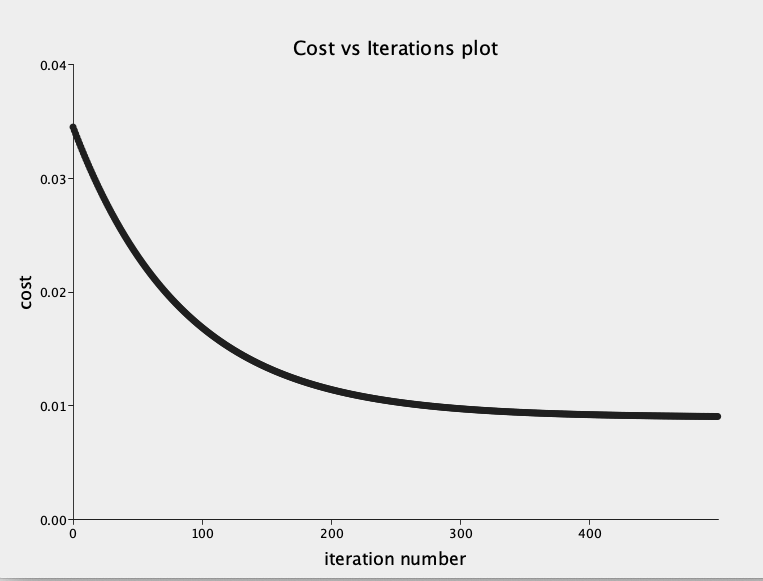
\includegraphics[width=\textwidth]{cost-iterations}
        \caption{A cost vs iterations plot where gradient descent has converged.}
        \label{fig:converged}
    \end{figure}

    We can tell gradient descent is working if it decreases on each iteration, and at the point where the cost seems to level off is when we can stop iterating.

    You can also use these plots to spot if something has gone wrong.

    \begin{figure}
        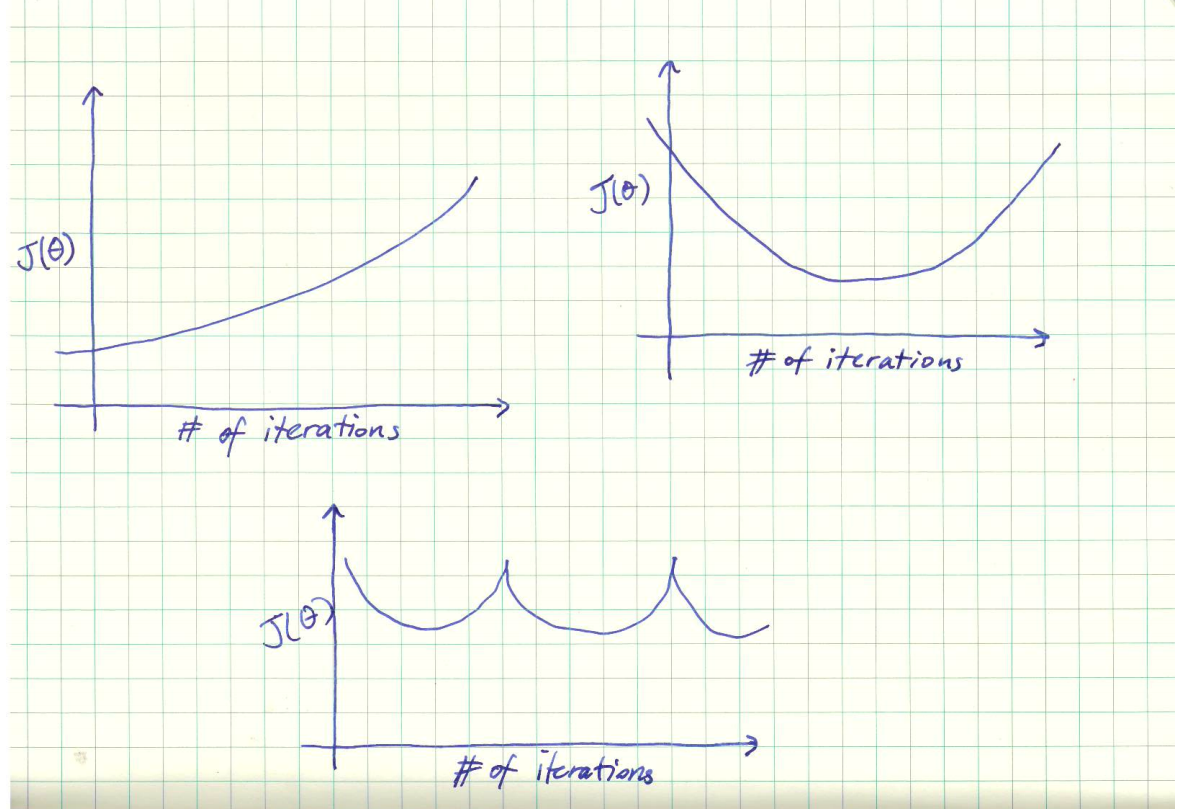
\includegraphics[width=\textwidth]{gd-diverged}
        \caption{Some cost vs iterations plots where gradient descent has diverged.}
        \label{fig:diverged}
    \end{figure}

    This usually means that our $\alpha$ is too big. We are probably overshooting the minimum. To go back to the analogy of getting to the lowest elevation, imagine that your steps are so large that it's like your landscape is actually a puddle, and you just keep stepping over it. 

    \subsubsection{Feature scaling}

    Imagine we are building a model where we and we have a feature $x_1$ which corresponds to age, and another $x_2$ which is annual income in pounds. In our dataset, the range of $x_1$ might be 18-65, and $x_2$ could be £10K-£500K. These features have very different ranges! If we tried to run gradient descent with this dataset as is, we'd end up trying to traverse a warped landscape. This is going to:
    \begin{itemize}
	\item Make our run of gradient descent \textit{slow}
	\item Make it harder to choose $alpha$ and the number of iterations needed
\end{itemize}
 
    
    \begin{figure}
    \centering
    \begin{subfigure}[b]{0.3\textwidth}
        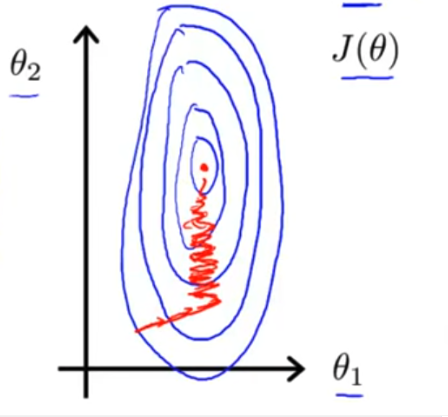
\includegraphics[width=\textwidth]{squashed}
        \caption{Gradient descent traversal when we our features vary greatly in range}
        \label{fig:squashed}
    \end{subfigure}
    ~ %add desired spacing between images, e. g. ~, \quad, \qquad, \hfill etc. 
      %(or a blank line to force the subfigure onto a new line)
    \begin{subfigure}[b]{0.3\textwidth}
        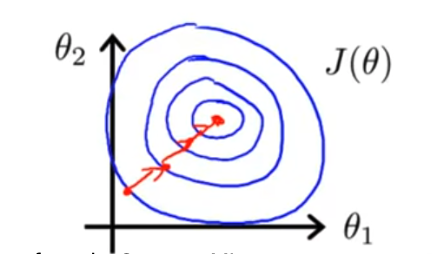
\includegraphics[width=\textwidth]{scaled}
        \caption{Gradient descent traversal when we've scaled our features}
        \label{fig:scaled}
    \end{subfigure}
    ~ %add desired spacing between images, e. g. ~, \quad, \qquad, \hfill etc. 
    %(or a blank line to force the subfigure onto a new line)
    \caption{Feature scaling for gradient descent. Figures from Andrew Ng's ML course on Coursera.}\label{fig:feature-scaling}
\end{figure}
    
    We can speed up gradient descent by ensuring that our data falls into similar ranges, while maintaining the shape of the data. In our case with one feature, LotArea, LotArea and selling price seem to have a linear relationship. After scaling LotArea, it will still have a linear relationship with selling price. 

    One common technique is \textit{mean normalisation}

    For some feature $x_i$, we find the mean $\mu_i$ and the range $s_i$ (max value - min value). Then for each point $j$ in $x_i$:
    \[
        x_i^{(j)} \leftarrow \frac{x_i^{(j)} - \mu_i^{(j)}}{s_i^{(j)}}
    \]

    and then for each $x_i^{(j)} $, $-0.5 \leq x_i^{(j)}  \leq 0.5$
    
    Mean normalisation isn't the only approach to take for feature scaling, but it will work well enough for our purposes here. \textit{Min-max scaling} and \textit{unit vector scaling} are also common, but we won't cover them here. 
    
    
    \begin{figure}
        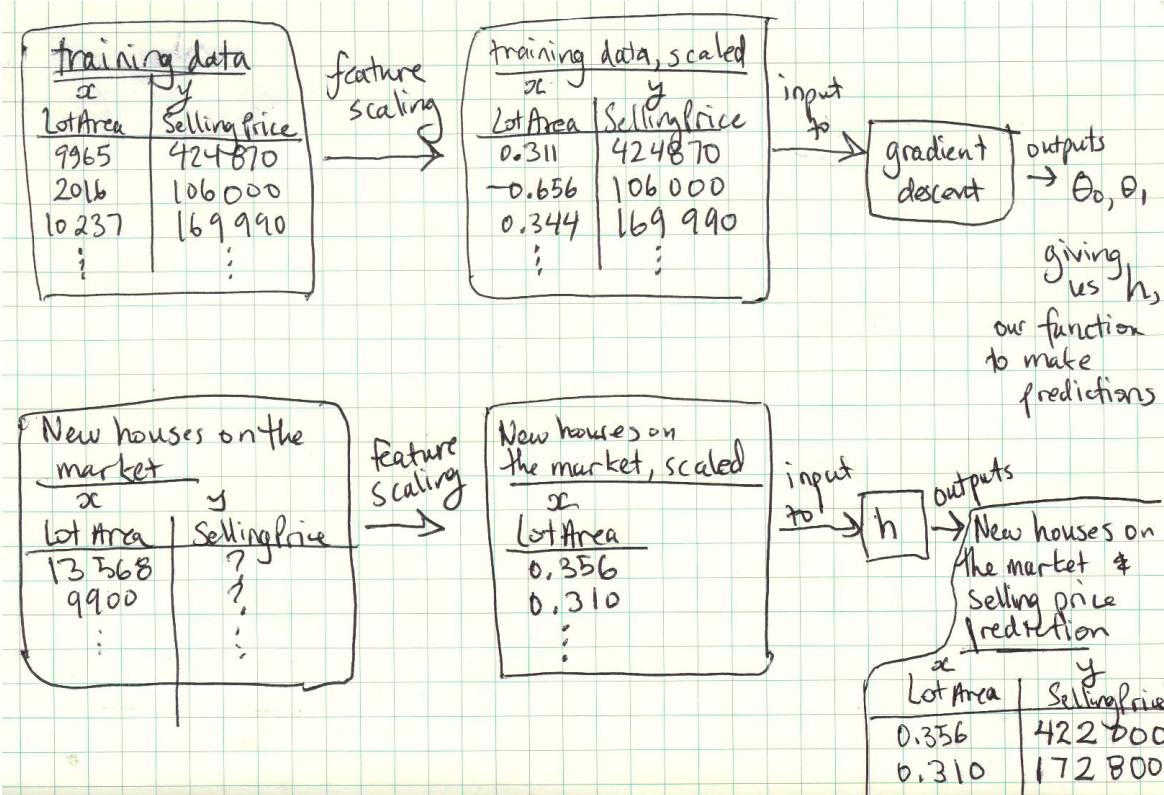
\includegraphics[width=\textwidth]{feature-scaling-data}
        \caption{Feature scaling when building a model and when making predictions }
        \label{fig:feature-scaling-data}
    \end{figure}
    
    We already know that feature scaling is a good idea if we need to run gradient descent. To do so, we apply a technique such as mean normalisation just to our $x$s.  So, when we run gradient descent, it is on data with scaled features. This means that when we want to make predictions, we must apply the same technique we used to scale our features when building the model, to the features in the new data we want to make predictions for. See Figure \ref{fig:feature-scaling-data}.

\end{document}